\documentclass[conference]{IEEEtran}
\IEEEoverridecommandlockouts
% The preceding line is only needed to identify funding in the first footnote. If that is unneeded, please comment it out.
\usepackage{cite}
\usepackage{amsmath,amssymb,amsfonts}
\usepackage{algorithmic}
\usepackage{graphicx}
\usepackage{textcomp}
\usepackage{xcolor}

% Increase Size
\usepackage{amsmath}
\usepackage{relsize}

% Write Optimization problems
\usepackage{amsmath}
\DeclareMathOperator*{\Max}{Max}
\DeclareMathOperator*{\Min}{Min}
\usepackage{optidef}


\def\BibTeX{{\rm B\kern-.05em{\sc i\kern-.025em b}\kern-.08em
    T\kern-.1667em\lower.7ex\hbox{E}\kern-.125emX}}

\begin{document}

\title{MA4740 - Introduction to Bayesian Statistics\\
}

\makeatletter
    \newcommand{\linebreakand}{%
      \end{@IEEEauthorhalign}
      \hfill\mbox{}\par
      \mbox{}\hfill\begin{@IEEEauthorhalign}
    }
\makeatother

\author{

\IEEEauthorblockN{1\textsuperscript{st} Krishna Teja Chilukuri}
\IEEEauthorblockA{\textit{Mathematics and Computing} \\
\textit{Indian Institute of Technology, Hyderabad} \\
Hyderabad, India \\
ma20btech11005@iith.ac.in
}

\and

\IEEEauthorblockN{2\textsuperscript{nd} Anita Dash}
\IEEEauthorblockA{\textit{Mathematics and Computing} \\
\textit{Indian Institute of Technology, Hyderabad} \\
Hyderabad, India \\
ma20btech11001@iith.ac.in
}

\linebreakand

\IEEEauthorblockN{3\textsuperscript{rd} KN Vardhan}
\IEEEauthorblockA{\textit{Mathematics and Computing} \\
\textit{Indian Institute of Technology, Hyderabad} \\
Hyderabad, India \\
ma20btech11006@iith.ac.in
}


}

% \and
% \IEEEauthorblockN{\textsuperscript{}}
% \IEEEauthorblockA{\textit{} \\
% \textit{}\\
% %  \\
% }


\maketitle

\begin{abstract}
% Here, the abstract
This report is based on a group project part of the MA4740 - Introduction to Bayesian Statistics course material. The primary goal of this project is to acquire a real-world data set (not synthetic) and execute Beta Binomial Bayesian Analysis and other approaches presented in class.
\end{abstract}

\section{Introduction}
The project includes collecting a real-life data set and applying the statistical methods while also performing a beta-binomial bayesian analysis. The real-life data set that we have taken is based on the stocks of MSFT (Microsoft Corp) from the past 2010 to 2022, for prior.  \\

The real-life data set, MSFT stocks have been taken from the Python3 \textit{yfinance} package. The data includes opening price, closing price, maximum price, minimum price and date. Amongst which, the attributes that are of our interest are closing price and date. 


\section{Prior Data}
As stated in the introduction, our prior data is on the stocks of MSFT from the year 2000 to 2022. The closing price of stocks' of MSFT on each and every day from all the years is taken into consideration. Based on this prior data, we try to guess if the stock of MSFT increases or decreases on a certain day after the year 2022. This data is taken as the training set. \\

We take the observation sample as either 0 or 1. 0 if the stock has decreased compared to the previous day and 1 if the stock has increased compared to the previous day. We choose a random variable $X$, where $X$ is the proportion of days the stock price increased in $n$ days, and $P(X = x)$ representing the probability of the proportion, $x$. \\

\newpage
\textbf{E.g.} Suppose in the past $n$ days, the MSFT stock has increased $k$ times, then
\begin{center}
    $x = \frac{k}{n}$
\end{center}

The plot between these proportions with its frequency gives us a near normal distribution. This is our prior data and it's probability mass function. The plot has been depicted below.


%     \begin{figure}[htp]
%     \begin{center}
% \includegraphics[width=0.7\textwidth]{FreqVsRise.png}
% \caption{Prior Data}
% \end{center}
% \end{figure}

\begin{figure}[htbp]
    \centerline{\includegraphics[scale=0.85]{Images/FreqVsRise.png}}
    \caption{Prior Data}
    \label{fig}
\end{figure}


\section{Applying the Methods}
    \par From the prior data collected, we apply MOM and MLE to fit the normal distribution of the above data. We have
    
    \begin{gather*}
        E[X] = \mu = \frac{1}{n}\Sigma x_{i} \\ 
        E[X^2] = \mu^2 + \sigma^2 = \frac{1}{n}\Sigma x_{i}^{2}
    \end{gather*}
    
    where, 
    \begin{itemize}
        \item $x_i$ are i.i.d realized values of $X$.
        \item $N(\mu,\sigma)$ is the normal distribution that fits the sample data.
    \end{itemize}
    
    \par Since our distribution is a normal distribution, the MOM and MLE yield the same result. Below is the plot depicted for MOM and MLE.
    
    \begin{figure}[htbp]
        \begin{center}
            \centerline{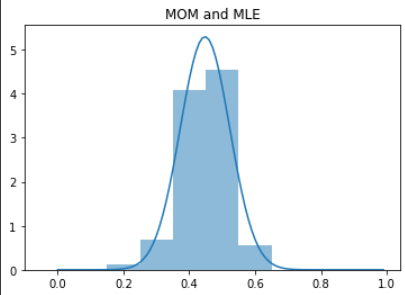
\includegraphics[scale=0.95]{Images/MOM_MLE.png}}
            \caption{MOM and MLE}
        \end{center}
    \end{figure}

    The calculations yield us the results \\
    \begin{align*}
        \textit{First moment = Mean }(\mu) = 0.4647727,\\
        \textit{Second moment} = 0.2235227,\\
        \textit{Variance }= 0.0075090,\\
        \textit{Standard Deviation }= 0.0866547,\\
    \end{align*}

\section{Beta-Bayesian}
    \subsection{Beta}
        \par We then apply the beta-binomial Bayesian analysis to this data. We try to fit the prior data distribution to a beta distribution. In a beta distribution, we get
        
        \[
            X \sim \Beta(\alpha, \beta)
        \]
    
        where,
        
        \begin{gather*}
            \textit{mean} = \frac{\alpha}{\alpha + \beta} \\
            \textit{var} = \frac{\alpha\beta}{(\alpha + \beta)^2(\alpha + \beta + 1)}
        \end{gather*}
            
        By calculating $\alpha$,$\beta$ using above MOM estimators we get,
        \begin{align*}
            \alpha = 19.05468607825279\\
            \beta =  23.50400363967223 \\ 
            \textit{Prior Mean} = 0.4477272727272727
        \end{align*}
        
        \par Given below is the plot of pdf of beta distribution of the prior data.
    
        \begin{figure}[htbp]
            \begin{center}
                \centerline{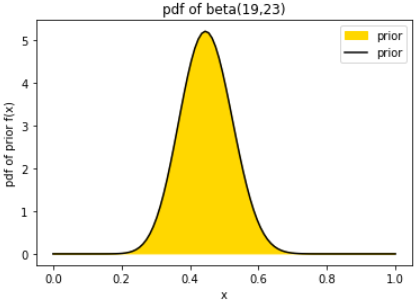
\includegraphics[scale=1]{Images/Pdf_beta_prior.png}}
                \caption{PDF of Beta(19,23)}
            \end{center}
        \end{figure}
        
    \subsection{Likelihood}
        Now we require a likelihood function to perform a beta-binomial analysis on the generated beta distribution. We choose $L \mid \pi \sim Bin(n,\pi)$ where,
        \begin{center}
            $n$: Number of days we are checking if the stock prize increased or decreased \\
            $\pi$: Probability of stock getting increased
        \end{center}
        
        After performing the calculations, we get the value of probability of stock increasing as $p = 0.4661354$. And the plot of the likelihood function and the prior distributions are  as follows
        \begin{figure}[htbp]
            \begin{center}
                \centerline{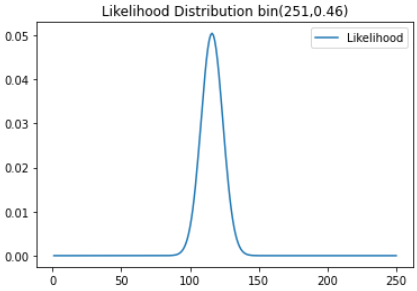
\includegraphics[scale=1]{Images/Likelihood_Dist.png}}
                \caption{Likelihood Distribution}
            \end{center}
        \end{figure}
        
        \begin{figure}[htbp]
            \begin{center}
                \centerline{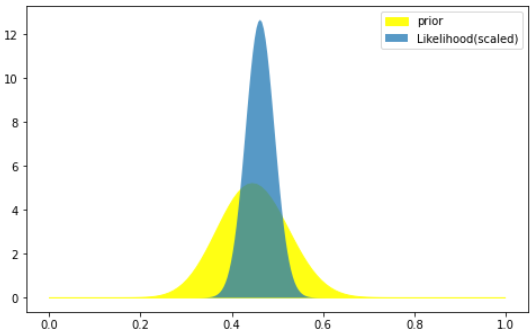
\includegraphics[scale=.8]{Images/Prior_Likelihood.png}}
                \caption{Combination of Prior and Likelihood(scaled)}
            \end{center}
        \end{figure}
    
    
    \subsection{Posterior}
        Finally, we find the posterior distribution from the prior data and the likelihood function. In a posterior distribution, we have 
        \[
            \pi \mid L = y \sim beta(\alpha', \beta')
        \] 
        where, 
        \begin{gather*}
            \alpha' = \alpha + y, \\
            \beta' =  \beta + n - y  
        \end{gather*}
        $y$ is the realized value of number of times stocks increased in $n$ days
        
        
        Thus, after performing the necessary calculations, we get 
        \begin{gather*}
            \alpha' = 135.0546860782528\\
            \beta' = 158.50400363967225\\
            \textit{Posterior mean} = 0.46006025646191656   
        \end{gather*}
    
        And the plot is as shown below
        \begin{figure}[htbp]
        \centering
          \centerline{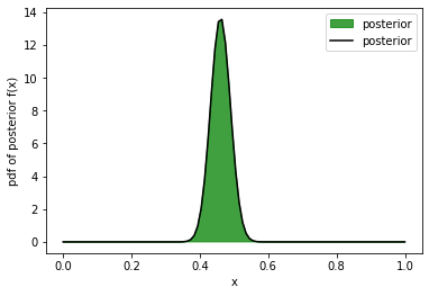
\includegraphics[scale=1]{Images/Posterior_Dist.png}}
        \end{figure}  
        
    \newpage
    \subsection{Conclusion}
        From the below combined plot we can see that the mean of our prior and posterior differ by 0.02 which is not that high. But the variance of prior and posterior differ by a lot.

        \begin{align*}
        \textit{Prior std} = 0.07534356570114019\\
        \textit{Post std} = 0.029039831153004316
        \end{align*}

        \begin{align*}
        \textit{Prior estimation of proportion} \approx \left (29.704\%, 59.841\% \right )\\
        \textit{Posterir estimation of proportion} \approx \left (40.198\%, 51.813\% \right )
        \end{align*}
        \begin{figure}[htbp]
        \centering
          \centerline{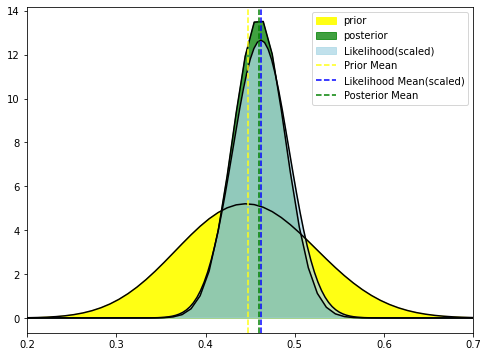
\includegraphics[scale=0.5]{Images/Final_Comb_Plot.png}}
          \caption{Combination of Prior, Data-Likelihood and Posterior Distribution}
        \end{figure}  

\end{document}
